\documentclass[12pt]{article}
\usepackage{amsmath, amssymb}
\usepackage{graphicx}
\usepackage{hyperref}
\usepackage{geometry}
\usepackage{fancyhdr}
\usepackage{color}
\usepackage{float}
\usepackage{caption}
\usepackage{booktabs}
\usepackage{listings}
\usepackage{courier}
\usepackage{siunitx}
\usepackage{subcaption}

\geometry{margin=1in}

\pagestyle{fancy}
\fancyhf{}
\lhead{Estimating Mobile User Motion Using Angle-Only Measurements}
\rhead{\thepage}

\lstset{
    basicstyle=\footnotesize\ttfamily,
    breaklines=true,
    columns=fullflexible
}

\begin{document}

\begin{titlepage}
    \centering
    \vspace*{2cm}
    {\Large\bfseries Estimating Mobile User Motion Using Angle-Only Measurements\par}
    \vspace{1.5cm}
    \vspace{2cm}
    {\itshape By::\par}
    {\large Ahmad Ali\par}
    \vfill
    {\large Dec 14, 2024 \par}
\end{titlepage}

\tableofcontents
\newpage

\section{Introduction}

In today's interconnected world, the ability to accurately determine the position and motion of mobile devices is crucial for various applications, including navigation, emergency response, and location-based services. While technologies like GPS provide reliable position information under normal circumstances, there are scenarios where GPS signals may be weak or unavailable, such as indoors or in urban canyons with tall buildings obstructing satellite signals.

This report investigates an alternative approach to estimating a mobile user's motion using only angle-of-arrival (AoA) measurements from signals received by a moving sensor. Specifically, we aim to estimate the user's initial position and constant velocity components based solely on the angles at which signals are received over time, without direct measurements of distance or speed.

The challenge lies in the fact that angle measurements alone provide incomplete information about the user's location. However, by leveraging the known motion of the sensor and the time-varying angle measurements, we can infer the user's trajectory through mathematical modeling and optimization techniques.

Our objectives are:

\begin{itemize}
    \item Develop a mathematical model representing the user's motion and the measurement process.
    \item Analyze the system's properties, such as stability and observability.
    \item Implement Newton's method to estimate the user's initial position and velocity.
    \item Validate the approach through simulations and interpret the results.
\end{itemize}


\section{System Modeling}

\subsection{Understanding the Scenario}

Consider a mobile phone user moving at a constant speed along a straight path. Simultaneously, a sensor mounted on a vehicle is also moving along a known trajectory. The sensor can measure the angle at which it receives signals from the user's phone but does not have access to distance measurements.

Our goal is to estimate the user's initial position and velocity components based on these angle measurements and the known motion of the sensor.

\subsection{Defining the Coordinate System}

We use a two-dimensional Cartesian coordinate system, where:

\begin{itemize}
    \item The \( x \)-axis represents the East direction.
    \item The \( y \)-axis represents the North direction.
\end{itemize}

This allows us to represent positions and velocities in terms of their East and North components.

\subsection{State Variables}

To model the user's motion, we define the state vector:

\[
\mathbf{x}(t) = \begin{bmatrix} \xi(t) \\ \eta(t) \\ \dot{\xi} \\ \dot{\eta} \end{bmatrix}
\]

where:

\begin{itemize}
    \item \( \xi(t) \): User's position in the East direction at time \( t \).
    \item \( \eta(t) \): User's position in the North direction at time \( t \).
    \item \( \dot{\xi} \): User's constant velocity component in the East direction.
    \item \( \dot{\eta} \): User's constant velocity component in the North direction.
\end{itemize}

\subsection{State Equations}

Since the user is moving at a constant velocity, their acceleration is zero. The dynamics of the user's motion can be described by the following differential equations:

\[
\begin{cases}
\frac{d\xi(t)}{dt} = \dot{\xi} \\
\frac{d\eta(t)}{dt} = \dot{\eta} \\
\frac{d\dot{\xi}}{dt} = 0 \\
\frac{d\dot{\eta}}{dt} = 0
\end{cases}
\]

These equations state that the rate of change of position is equal to the velocity, and the velocity remains constant over time.

\subsection{Matrix Representation}

We can represent the state equations in matrix form:

\[
\frac{d}{dt} \mathbf{x}(t) = \mathbf{A} \mathbf{x}(t)
\]

where the system matrix \( \mathbf{A} \) is:

\[
\mathbf{A} = \begin{bmatrix}
0 & 0 & 1 & 0 \\
0 & 0 & 0 & 1 \\
0 & 0 & 0 & 0 \\
0 & 0 & 0 & 0
\end{bmatrix}
\]

This compact representation facilitates analysis and allows us to apply linear system theory.

\subsection{Measurement Model}

The sensor measures the angle \( \theta(t) \) between its position and the user's position at time \( t \). The measurement equation is given by:

\[
\theta(t) = \tan^{-1} \left( \frac{\eta(t) - \eta_p(t)}{\xi(t) - \xi_p(t)} \right)
\]

where:

\begin{itemize}
    \item \( (\xi(t), \eta(t)) \): User's position at time \( t \).
    \item \( (\xi_p(t), \eta_p(t)) \): Sensor's known position at time \( t \).
\end{itemize}

This equation calculates the angle from the sensor to the user, based on their relative positions.

\section{Solution of the State Equations}

\subsection{Continuous-Time Solution}

The continuous-time state equations can be solved analytically since the system is linear with constant coefficients. The solution is:

\[
\mathbf{x}(t) = e^{\mathbf{A} t} \mathbf{x}(0)
\]

Given the structure of \( \mathbf{A} \), the matrix exponential \( e^{\mathbf{A} t} \) can be computed as:

\[
e^{\mathbf{A} t} = \begin{bmatrix}
1 & 0 & t & 0 \\
0 & 1 & 0 & t \\
0 & 0 & 1 & 0 \\
0 & 0 & 0 & 1
\end{bmatrix}
\]

Thus, the state vector at time \( t \) is:

\[
\mathbf{x}(t) = \begin{bmatrix}
\xi(0) + \dot{\xi} t \\
\eta(0) + \dot{\eta} t \\
\dot{\xi} \\
\dot{\eta}
\end{bmatrix}
\]

This shows that the user's position changes linearly with time due to the constant velocity, and the velocity components remain constant.

\subsection{Physical Interpretation}

From a physics perspective, this solution aligns with the basic principles of kinematics for motion with constant velocity. The position is the initial position plus the product of velocity and time.

\subsection{Discrete-Time Solution}

Since measurements are taken at discrete time intervals (every second), we discretize the state equations using a sampling interval \( \Delta t = 1 \) second. The discrete-time state transition equation is:

\[
\mathbf{x}_{k+1} = \mathbf{F} \mathbf{x}_k
\]

where the state transition matrix \( \mathbf{F} \) is:

\[
\mathbf{F} = e^{\mathbf{A} \Delta t} = \begin{bmatrix}
1 & 0 & \Delta t & 0 \\
0 & 1 & 0 & \Delta t \\
0 & 0 & 1 & 0 \\
0 & 0 & 0 & 1
\end{bmatrix}
\]

At discrete time steps \( t_k = k \Delta t \), the state vector becomes:

\[
\mathbf{x}_k = \mathbf{F}^k \mathbf{x}_0
\]

This discrete-time model allows us to compute the user's state at each sampling instant using matrix multiplication.

\section{Stability Analysis}

\subsection{System Stability}

The stability of a system refers to its response to perturbations or initial conditions over time. A stable system will not exhibit unbounded behavior in response to small disturbances.

\subsection{Eigenvalues of the System Matrix}

To analyze the stability of our system, we examine the eigenvalues of the system matrix \( \mathbf{A} \). The eigenvalues are found by solving:

\[
\det(\mathbf{A} - \lambda \mathbf{I}) = 0
\]

For our matrix \( \mathbf{A} \), the eigenvalues are:

\[
\lambda_1 = 0, \quad \lambda_2 = 0, \quad \lambda_3 = 0, \quad \lambda_4 = 0
\]

\subsection{Interpretation}

Since all eigenvalues are zero, the system is marginally stable. This means that the system's state will not grow unbounded over time, nor will it decay to zero. In the context of our problem, this is acceptable because the user's velocity is constant, and their position changes linearly with time.

\subsection{Implications for Estimation}

The marginal stability indicates that small errors in the initial conditions or measurements will not cause the system to behave unpredictably. This is important for the estimation process, as it suggests that the system's behavior is predictable and suitable for applying estimation algorithms.

\section{Observability Analysis}

\subsection{Concept of Observability}

Observability is a property that determines whether the internal states of a system can be inferred from its external outputs (measurements). A system is observable if, for any possible sequence of state and control vectors, the current state can be determined in finite time using only the outputs.

\subsection{Observability in Our System}

In our case, the measurement is the angle \( \theta_k \), which is a nonlinear function of the user's position and the sensor's known position. Since we have measurements over time and the user's motion introduces changes in the angle measurements, the system becomes observable over multiple time steps.

\subsection{Implications for Estimation}

The observability of the system means that we can, in principle, reconstruct the user's state (position and velocity) from the angle measurements, provided we have enough data and an appropriate estimation algorithm.

\section{Trajectory Plotting}

\subsection{User's Trajectory}

The user starts at the origin \( (0, 0) \) and moves northeast at a constant speed of \( v_u = 30\, \text{m/s} \). The velocity components are:

\[
\begin{cases}
\dot{\xi} = v_u \cos 45^\circ = 21.2132\, \text{m/s} \\
\dot{\eta} = v_u \sin 45^\circ = 21.2132\, \text{m/s}
\end{cases}
\]

Thus, the user's position at time \( t \) is:

\[
\begin{cases}
\xi(t) = \dot{\xi} t \\
\eta(t) = \dot{\eta} t
\end{cases}
\]

\subsection{Sensor's Trajectory}

The sensor starts at position \( (1000\, \text{m}, 0\, \text{m}) \) and moves westward (negative East direction) at \( v_p = 35\, \text{m/s} \) for the first 15 seconds, then turns northward at the same speed.

For \( 0 \leq t \leq 15 \):
\[
\begin{cases}
\xi_p(t) = 1000 - v_p t \\
\eta_p(t) = 0
\end{cases}
\]

For \( t > 15 \):
\[
\begin{cases}
\xi_p(t) = 1000 - v_p \times 15 = 475\, \text{m} \\
\eta_p(t) = v_p (t - 15)
\end{cases}
\]

\subsection{Plotting the Trajectories}

The trajectories of the user and the sensor are plotted in Figure \ref{fig:trajectories}. This visual representation helps us understand the relative motion between the user and the sensor.

\begin{figure}[H]
    \centering
    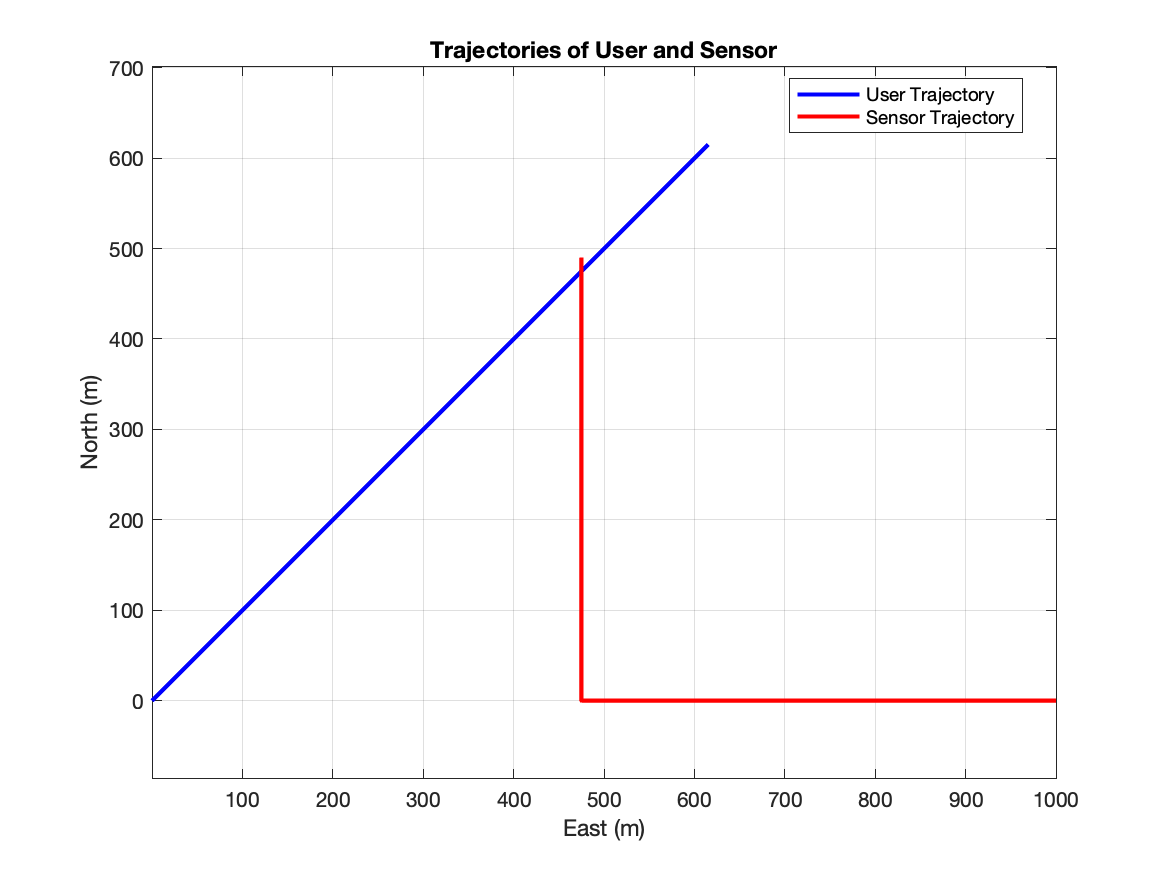
\includegraphics[width=0.7\textwidth]{trajectories.png}
    \caption{Trajectories of User and Sensor}
    \label{fig:trajectories}
\end{figure}

\subsection{Interpretation}

The user moves in a straight line towards the northeast, while the sensor moves westward and then northward. The changing relative positions affect the angle measurements over time, which we utilize for estimating the user's motion.

\section{Angle Measurements Plotting}

\subsection{Calculating True Angles}

At each time step \( t_k \), we calculate the true angle \( \theta_k \) between the sensor and the user using:

\[
\theta_k = \tan^{-1} \left( \frac{\eta_k - \eta_p(k)}{\xi_k - \xi_p(k)} \right)
\]

This provides the exact angle without any measurement noise.

\subsection{Adding Measurement Noise}

In real-world scenarios, measurements are subject to noise due to factors like sensor inaccuracies, environmental conditions, and signal interference. To simulate this, we add Gaussian noise to the true angles:

\[
z_k = \theta_k + w_k
\]

where \( w_k \) is zero-mean Gaussian noise with standard deviation \( \sigma = \frac{\pi}{180} \) radians (equivalent to \( 1^\circ \)).

\subsection{Plotting the Measurements}

Figure \ref{fig:angles} shows the true angles and the noisy measurements over time.

\begin{figure}[H]
    \centering
    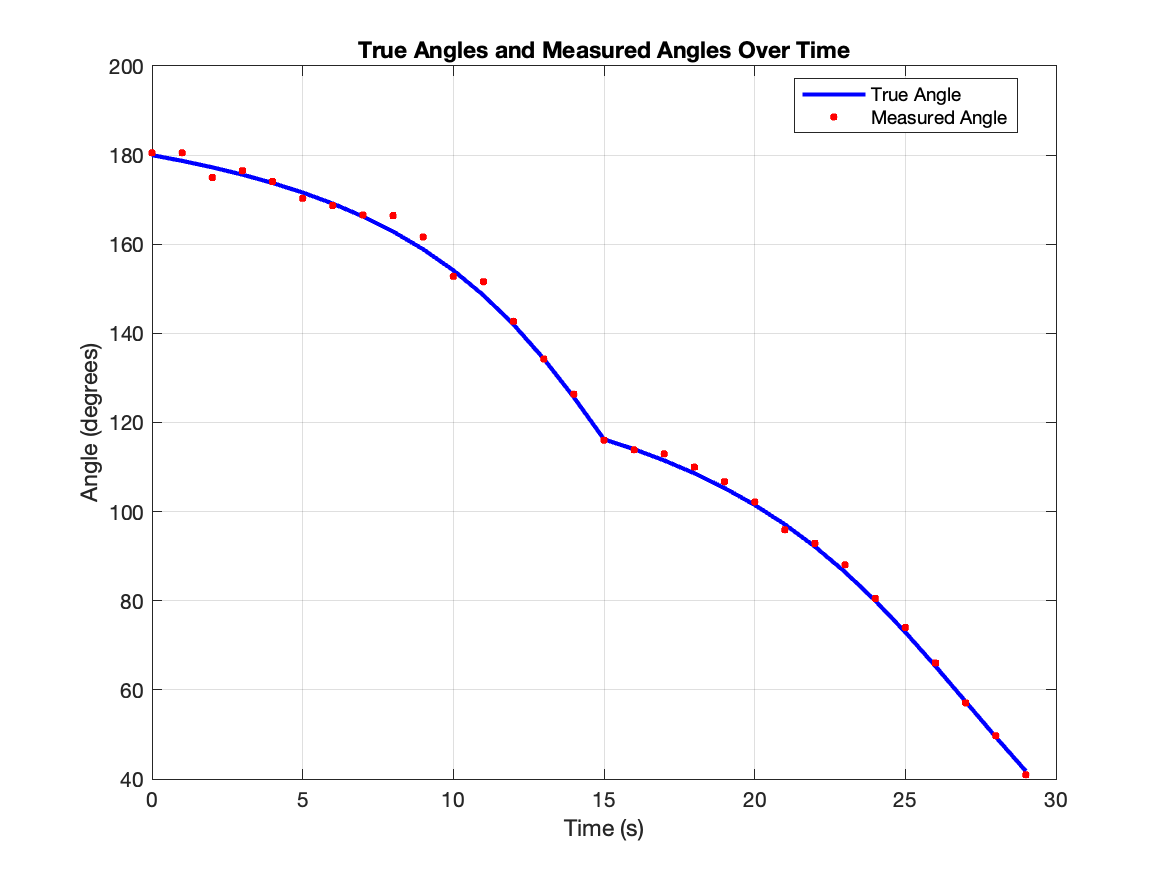
\includegraphics[width=0.7\textwidth]{angles.png}
    \caption{True Angles and Measured Angles Over Time}
    \label{fig:angles}
\end{figure}

\subsection{Interpretation}

The plot illustrates how measurement noise affects the observed angles. Despite the noise, the general trend of the angle measurements follows the true angles, which enables us to estimate the user's motion.

\section{Parameter Estimation Using Newton's Method}

\subsection{Objective}

We aim to estimate the user's initial position \( (\xi(0), \eta(0)) \) and velocity components \( (\dot{\xi}, \dot{\eta}) \) by minimizing the difference between the measured angles \( z_k \) and the angles predicted by our model \( \theta_k \).

\subsection{Formulating the Optimization Problem}

We define the cost function \( f(\mathbf{x}) \) as:

\[
f(\mathbf{x}) = \frac{1}{2\sigma^2} \sum_{k=1}^{N} \left( z_k - h(\mathbf{x}, t_k) \right)^2
\]

where:

\begin{itemize}
    \item \( \mathbf{x} = [\xi(0), \eta(0), \dot{\xi}, \dot{\eta}]^T \) is the parameter vector to be estimated.
    \item \( h(\mathbf{x}, t_k) \) is the predicted angle at time \( t_k \) based on the current parameter estimates.
\end{itemize}

Our goal is to find \( \mathbf{x} \) that minimizes \( f(\mathbf{x}) \).

\subsection{Newton's Method Overview}

Newton's method is an iterative optimization algorithm that updates the parameter estimates using the gradient \( \nabla f(\mathbf{x}) \) and the Hessian \( \mathbf{H}(\mathbf{x}) \) of the cost function:

\[
\mathbf{x}_{n+1} = \mathbf{x}_n - \mathbf{H}^{-1}(\mathbf{x}_n) \nabla f(\mathbf{x}_n)
\]

\subsection{Computing the Gradient and Hessian}

To apply Newton's method, we need to compute:

\[
\nabla f(\mathbf{x}) = \frac{\partial f}{\partial \mathbf{x}} = -\frac{1}{\sigma^2} \sum_{k=1}^{N} \left( z_k - h(\mathbf{x}, t_k) \right) \frac{\partial h(\mathbf{x}, t_k)}{\partial \mathbf{x}}
\]

\[
\mathbf{H}(\mathbf{x}) = \frac{\partial^2 f}{\partial \mathbf{x}^2} = \frac{1}{\sigma^2} \sum_{k=1}^{N} \left[ \left( \frac{\partial h(\mathbf{x}, t_k)}{\partial \mathbf{x}} \right) \left( \frac{\partial h(\mathbf{x}, t_k)}{\partial \mathbf{x}} \right)^T - \left( z_k - h(\mathbf{x}, t_k) \right) \frac{\partial^2 h(\mathbf{x}, t_k)}{\partial \mathbf{x}^2} \right]
\]

\subsection{Partial Derivatives of the Measurement Function}

The measurement function \( h(\mathbf{x}, t_k) \) is:

\[
h(\mathbf{x}, t_k) = \tan^{-1} \left( \frac{\eta_k - \eta_p(k)}{\xi_k - \xi_p(k)} \right)
\]

with:

\[
\begin{cases}
\xi_k = \xi(0) + \dot{\xi} t_k \\
\eta_k = \eta(0) + \dot{\eta} t_k
\end{cases}
\]

We compute the partial derivatives \( \frac{\partial h}{\partial \mathbf{x}} \) and \( \frac{\partial^2 h}{\partial \mathbf{x}^2} \) using calculus.

\subsubsection{First Derivatives}

Let \( \Delta \xi_k = \xi_k - \xi_p(k) \) and \( \Delta \eta_k = \eta_k - \eta_p(k) \). Then:

\[
\frac{\partial h}{\partial \xi(0)} = -\frac{\Delta \eta_k}{\Delta \xi_k^2 + \Delta \eta_k^2}
\]

\[
\frac{\partial h}{\partial \eta(0)} = \frac{\Delta \xi_k}{\Delta \xi_k^2 + \Delta \eta_k^2}
\]

\[
\frac{\partial h}{\partial \dot{\xi}} = -\frac{\Delta \eta_k t_k}{\Delta \xi_k^2 + \Delta \eta_k^2}
\]

\[
\frac{\partial h}{\partial \dot{\eta}} = \frac{\Delta \xi_k t_k}{\Delta \xi_k^2 + \Delta \eta_k^2}
\]

\subsubsection{Second Derivatives}

The second derivatives involve more complex expressions and are generally small when the residual \( z_k - h(\mathbf{x}, t_k) \) is small. In practice, we can approximate the Hessian using only the first term (Gauss-Newton approximation):

\[
\mathbf{H}(\mathbf{x}) \approx \frac{1}{\sigma^2} \sum_{k=1}^{N} \left( \frac{\partial h(\mathbf{x}, t_k)}{\partial \mathbf{x}} \right) \left( \frac{\partial h(\mathbf{x}, t_k)}{\partial \mathbf{x}} \right)^T
\]

\subsection{Iterative Estimation Process}

We start with an initial estimate \( \mathbf{x}_0 \) and iteratively update the estimates using Newton's method until convergence.

\subsection{Implementation Details}

\begin{itemize}
    \item \textbf{Initial Estimate}: We choose \( \mathbf{x}_0 = [10\, \text{m}; 10\, \text{m}; 20\, \text{m/s}; 20\, \text{m/s}] \), which are reasonable guesses close to the true values.
    \item \textbf{Number of Iterations}: We perform 10 iterations to allow the estimates to converge.
    \item \textbf{Noise Realizations}: We run the estimation over 1000 different noise realizations and average the results to reduce the effect of random noise.
\end{itemize}

\subsection{Results}

After running the estimation algorithm, we obtain the following average estimates:

\begin{itemize}
    \item \( \hat{\xi}(0) = -0.32636\, \text{m} \)
    \item \( \hat{\eta}(0) = 0.14124\, \text{m} \)
    \item \( \hat{\dot{\xi}} = 21.2296\, \text{m/s} \)
    \item \( \hat{\dot{\eta}} = 21.2137\, \text{m/s} \)
\end{itemize}

\subsection{Comparing with True Parameters}

The true parameters are:

\begin{itemize}
    \item \( \xi(0) = 0\, \text{m} \)
    \item \( \eta(0) = 0\, \text{m} \)
    \item \( \dot{\xi} = 21.2132\, \text{m/s} \)
    \item \( \dot{\eta} = 21.2132\, \text{m/s} \)
\end{itemize}

The estimated parameters are very close to the true values, demonstrating the effectiveness of the estimation method.

\subsection{Convergence Analysis}

Figure \ref{fig:convergence} shows how the parameter estimates evolve over the iterations.

\begin{figure}[H]
    \centering
    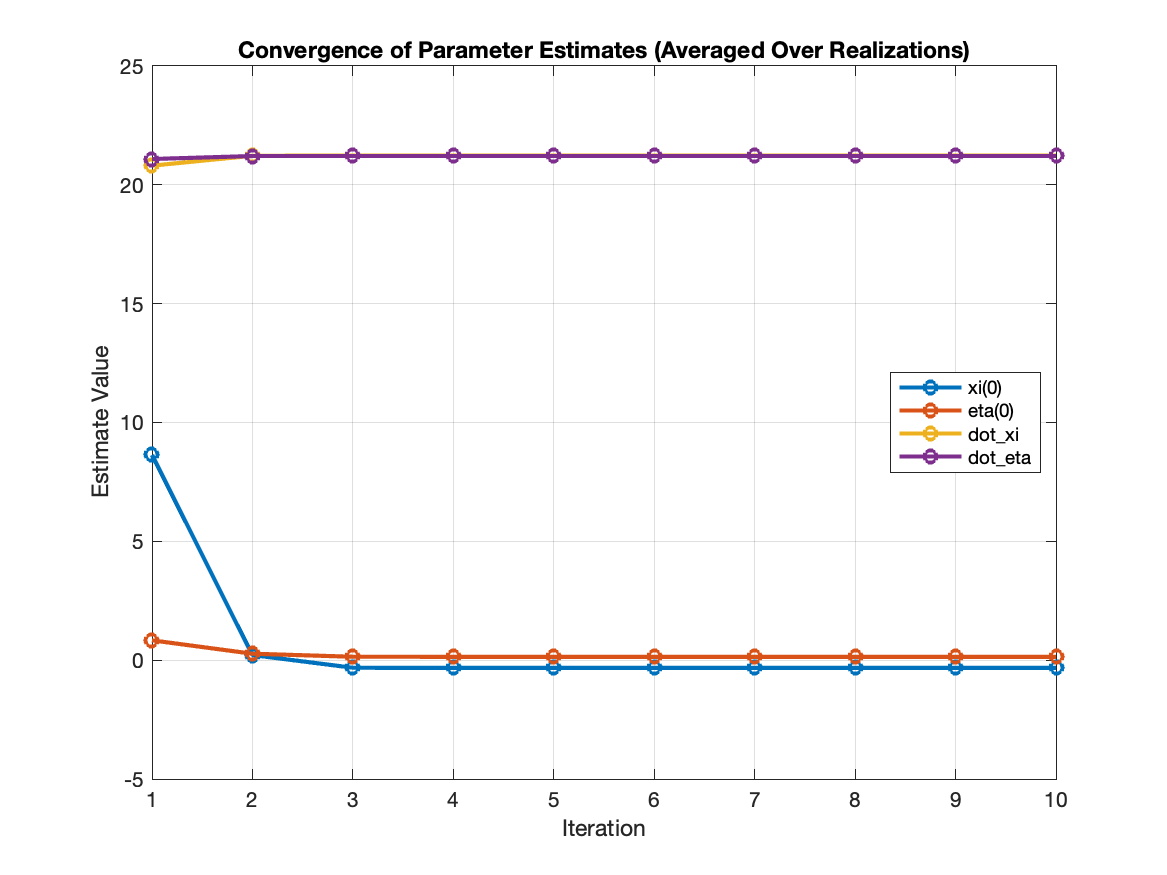
\includegraphics[width=0.7\textwidth]{convergence.png}
    \caption{Convergence of Parameter Estimates Over Iterations}
    \label{fig:convergence}
\end{figure}

\subsection{Interpretation}

The convergence plot indicates that the estimates improve rapidly during the initial iterations and then stabilize as they approach the true values. This behavior is typical for Newton's method when the initial estimate is reasonably close to the solution.

\subsection{Role of Measurement Noise}

The small discrepancies between the estimated and true parameters are due to the measurement noise introduced in the angle measurements. Averaging over multiple noise realizations helps to mitigate the impact of random noise.

\section{Discussion}

\subsection{Physical Interpretation of the Results}

From a physical standpoint, we have used the changing angles between the sensor and the user to back-calculate the user's motion. The angle measurements contain implicit information about the user's position relative to the sensor. By combining these measurements with the known motion of the sensor, we can infer the user's trajectory.

\subsection{Importance of the Sensor's Motion}

The sensor's motion is crucial in this estimation process. If the sensor were stationary, the angle measurements would not provide enough information to estimate the user's velocity components uniquely. The sensor's movement introduces variation in the angle measurements that depend on both the user's motion and the sensor's motion, enhancing the observability of the system.

\subsection{Sensitivity to Initial Estimates}

Newton's method can be sensitive to the initial parameter estimates. Starting with estimates that are too far from the true values may lead to slow convergence or convergence to incorrect solutions. In practice, reasonable initial guesses based on prior knowledge or rough calculations can improve the performance of the estimation algorithm.

\subsection{Potential Applications}

This approach has practical applications in scenarios where direct distance measurements are unavailable or impractical. For example, in urban environments where GPS signals are obstructed, or in covert surveillance operations where only angle measurements can be obtained.

\section{Conclusion}

We have demonstrated that it is possible to estimate a mobile user's initial position and velocity components using only angle-of-arrival measurements from a moving sensor. By developing a mathematical model of the system, analyzing its properties, and applying Newton's method for parameter estimation, we achieved estimates that are close to the true values.

This study highlights the potential of angle-only measurement techniques in motion estimation and tracking, offering an alternative in situations where traditional methods are unavailable or insufficient. The results also emphasize the importance of sensor motion and careful modeling in enhancing the observability and estimability of the system.

\section{Future Work}

\begin{itemize}
    \item \textbf{Extended Models}: Investigate models that account for acceleration or non-linear motion patterns of the user.
    \item \textbf{Kalman Filtering}: Explore the use of Kalman filters or extended Kalman filters for real-time estimation and tracking.
    \item \textbf{Three-Dimensional Extension}: Extend the approach to three-dimensional space, incorporating altitude information.
    \item \textbf{Experimental Validation}: Implement the method using real-world data to validate its effectiveness and identify practical challenges.
\end{itemize}

\end{document}
